\newpage
\section{Planung eines Business Intelligence Prozesses für ein Mining Rechenzentrum} \label{toc:planungeinesbiprozessesfuereinminingrechenzentrum}

Im folgenden Kapitel wird evaluiert, ob ein \ac{BI} Prozess unter den Bedingungen, die in vorhergehenden Kapitel erarbeitet
worden sind, betrieblich durchführbar ist. Für diese Prüfung existieren unter anderem zwei Ansätze, die in der Veröffentlichung
"`Business Intelligence Stategy"' von John Boyer et al. beschrieben werden:\footcite[Vgl.][S. 102]{boyer2010business}

\begin{itemize}
    \item \textbf{Analyse der Stakeholder: } In Kapitel \ref{toc:stakeholderanalyse} werden die Stakeholder des betreffenden
    \ac{BI} Prozesses identifiziert. Damit ist es möglich, technologische Ansätze zur Realisierung zu identifizieren
    und zu analyieren, ob dieser Prozess ausreichend Unterstützung innerhalb des Betriebes erfahren wird. Diese Unterstützung
    hängt in erster Linie davon ab, wie viele Stakeholder vom Mehrwert eines \ac{BI} Prozesses profitieren.
    Anhand dessen werden in Kapitel \ref{toc:datenpraesentation}
    die passenden Präsentationsformen der Daten identifiziert.\footcite[Vgl.][S. 102]{boyer2010business}
    \item \textbf{Technologische Umgebung: }Es wird die technologische Umgebung innerhalb des Betriebes analysiert.
    Dadurch können Komponenten identifiziert werden, die bereits exisitieren und nur integriert werden
    müssen.\footcite[Vgl.][S. 102]{boyer2010business} Zusätzlich
    kann die Argumentation aus Kapitel \ref{toc:ansatzmoeglichkeitenfuerbusinessintelligence} damit erweitert bzw. unterstützt
    werden. Als technologische Basis für die Realisierung wird die Google Cloud in Betracht gezogen, da diese innerhalb der
    Genesis Group stark genutzt wird.
\end{itemize}

Um aussagekräftige Ergebnisse auf diese beiden Punkte zu erhalten, wird eine kleine Fallstudie in Kapitel
\ref{toc:fallstudiendesign} konzipiert, damit die betriebliche Umsetzbarkeit geprüft werden kann. Gegen Ende des Kapitels werden die
Ergebnisse aus dieser Studie kurz zusammengefasst und evaluiert. Eine kritische Bewertung der gesamten Argumentation findet
im Fazit dieser Arbeit statt.

\subsection{Design und Methodik der Fallstudie} \label{toc:fallstudiendesign}

In diesem Teil wird der prinzipielle Aufbau der Fallstudie beschrieben. Für das Design der Fallstudie wird das Vorgehen von
Göthlich verwendet.\footcite[Vgl.][]{gothlich2003fallstudien} Die Herangehensweise ist zusammenfassend in Abbildung
\ref{figure:casestudydesign} dargestellt.

\begin{figure}[H]
    \caption{Aufbau und Design einer Fallstudie}
    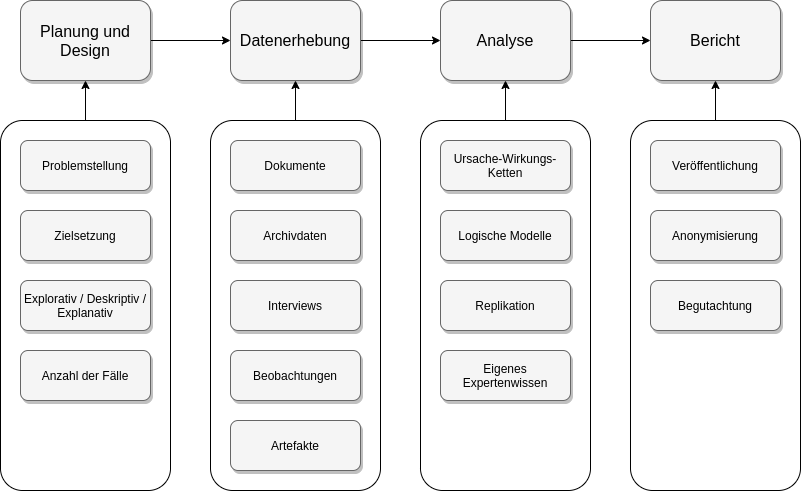
\includegraphics[width=0.8\textwidth]{casestudydesign}
    \label{figure:casestudydesign}
    \\
    \cite[Quelle: In Anlehnung an][S. 8ff]{gothlich2003fallstudien}
\end{figure}

Im Folgenden werden die einzelnen Schritte beschrieben und dadurch das Design
festgelegt:\footcite[Vgl.][S. 8ff]{gothlich2003fallstudien}
\begin{itemize}
    \item \textbf{Planung und Design: }Im ersten Schritt werden die Problemstellung und die Ziele genannt, die durch die Fallstudie
    abgedeckt werden sollen. Die Problemstellung ist bereits in Kapitel \ref{toc:motivation} und \ref{toc:hypothesenundabgrenzungderarbeit}
    hinreichend beschrieben. Das Ziel dieser Fallstudie ist es, die Beantwortung der Hypothesen in Kapitel \ref{toc:ansatzmoeglichkeitenfuerbusinessintelligence}
    durch eine Prüfung der betrieblichen Umsetzbarkeit zu erweitern. Es soll die Belastbarkeit der Aussagen dieser Arbeit zu vergrößert werden, indem
    auf Basis der theoretischen Analyse eine Anwendung in der Praxis geplant wird.
    Daher ist das Forschungsziel in der Studie explorativer Natur.\footcite[Vgl.][S. 8]{gothlich2003fallstudien}
    Diese Fallstudie wird ein einziges Mal in dieser Form durchgeführt (``Single-Case''). Dadurch entfällt eine mögliche Replikation dieser Studie.\footcite[Vgl.][S. 8f]{gothlich2003fallstudien}
    \item \textbf{Datenerhebung: }In diesem Schritt werden die Datenquellen definiert, die für die Fallstudie zur Verfügung stehen. Neben den
    Datenquellen, die in Kapitel \ref{toc:klassifizierungderdaten} beschrieben sind, stehen zusätzlich noch interne Dokumente der Genesis
    Group zur Verfügung. Diese sind im Anhang zu dieser Arbeit zu finden. Daher basiert die Fallstudie aus Dokumenten und Artefakten.\footcite[Vgl.][Tabelle 1 ]{gothlich2003fallstudien}
    \item \textbf{Analyse: }Es wird im Zuge der Analyse ein Modell für einen beispielhaften \ac{BI} Prozess errichtet,
    der innerhalb der Genesis Group Anwendung finden kann. Anhand dessen wird geprüft, ob die Einführung möglich ist und dadurch die
    Hypothesen dieser Arbeit unterstützt werden können. Dafür werden "`Ursache-Wirkungs-Ketten"' und logische Modelle verwendet.\footcite[Vgl.][S. 11]{gothlich2003fallstudien}
    Bei diesen beiden Analysemodellen wird stark Bezug auf ein betriebliches Umfeld genommen.
    \item \textbf{Bericht: }Der letzte Schritt beschäftigt sich mit der Veröffentlichung dieser Fallstudie. Da diese Fallstudie im Rahmen
    dieser Arbeit stattfindet, ist eine Veröffentlichung bereits vorgesehen. Eine Begutachtung ist dennoch sinnvoll und wird im Zuge
    der nachträglichen innerbetrieblichen Evaluation vorgenommen.
\end{itemize}

Im Folgenden wird eine Stakeholderanalyse am Beispiel der Genesis Group vorgenommen. Mit Hilfe der Ergebnisse dieser Analyse und dem zusätzlichen
theoretischen Wissen aus dieser Arbeit wird in Kapitel \ref{toc:planungdesbiprozesses} ein bespielhafter \ac{BI} Prozess erstellt und dieser
in Kapitel \ref{toc:abschliessendebewertung} abschließend auf dessen Durchführbarkeit geprüft.

\subsection{Stakeholderanalyse für einen internen Business Intelligence Prozess} \label{toc:stakeholderanalyse}

Die folgende Stakeholderanalyse basiert in erster Linie auf der Veröffentlichung "`A Stakeholder Model of Business
Intelligence"' von Claire A. Simmers.\footcite[Vgl.][]{simmers2004stakeholder} Diese Arbeit beschäftigt sich mit
der Stakeholderanalyse im Bereich \ac{BI} und wird für die vorliegende Analyse verwendet. Ausgehend von
Abbildung 14.2 in dieser Veröffentlichung wird die Analyse der Stakeholder betrieben und werden damit die einzelnen Personen oder Gruppen identifiziert,
die Interesse an der erfolgreichen Einführung eines \ac{BI} Prozesses haben.\footcite[Vgl.][Abb. 14.2]{simmers2004stakeholder}

Die folgenden Stakeholder können für die Optimierung von Kryptomining Rechenzentren im Cloud Mining Umfeld identifiziert
werden:\footcite[Vgl.][Abb. 14.2]{simmers2004stakeholder}\footcite[Vgl.][S. 52]{reed2009s}
\begin{itemize}
    \item \textbf{Eigentümer des Unternehmens: }Die Eigentümer der Genesis Group sind für die strategischen Entscheidungen verantwortlich und
    haben ein Interesse an der erfolgreichen Einführung
    eines solchen \ac{BI} Prozesses. Dies können Gründe, wie die Verbesserung des Mining Ertrags, Vorteile am Cloud Mining Markt
    durch eine höhere Effizienz der Rechenzentren und eine Entscheidungsunterstützung hinsichtlich des Neu- oder Ausbaus von Mining
    Rechenzentren, sein. Daher sind vor allen \ac{HT0.1} und \ac{HT0.3} für diese Personen relevant.
    \item \textbf{Arbeitnehmer: }Eine weitere relevante Gruppe sind die Arbeitnehmer der Genesis Group. Diese profitieren
    durch die Einführung von \ac{BI} gerade in Hinblick auf die Zeitersparnis, Prozessoptimierung und
    Entscheidungsunterstützung (Vgl. Kapitel \ref{toc:strategischermehrwert}). Diese Gruppe ist in die folgenden Untergruppen
    aufteilbar:
    \begin{itemize}
        \item Geschäftsführung: Diese Gruppe hat maßgeblich Interesse an der Entscheidungsunterstützung, die ein \ac{BI} Prozess
        bietet. Taktische Entscheidungen, die den Betrieb von Rechenzentren betreffen, werden von dieser Gruppe
        getätigt. Aus diesem Grund hat die Geschäftsführung Interesse an einer korrekten Darstellung des Cashflows eines Rechenzentrums, was
        in \ac{HT0.3} geprüft wird.
        \item Management der Rechenzentren: Diese Gruppe verwaltet die existierenden Rechenzentren und ist im Bereich
        der operativen Entscheidungen anzutreffen. Sie hat Interesse am Betrieb möglichst effizienter Hardware (\ac{HT0.2}),
        am Cashflow eines Rechenzentrums (\ac{HT0.3}) und an der Optimierung der personellen Ausstattung eines Mining Rechenzentrums
        (\ac{HT0.4}).
        \item Controlling: Die Controlling Abteilung übernimmt die finanzielle Überwachung der Rechenzentren. Daher hat diese
        Gruppe von Personen unmittelbares Interesse an einem schnellen und korrekten Zugang zu den finanziellen Daten, aus denen
        letztendlich der Cashflow berechnet werden kann (\ac{HT0.3}).
        \item IT: Die technischen Abteilungen sind in erster Linie die Wartung und den Betrieb der vorhandenen Hardware zuständig.
        Daher benötigen diese vor allem technische \acp{KPI}, die durch \ac{HT0.2} abgedeckt werden. Durch die Verfügbarkeit
        dieser Daten kann die Effizienz der Hardware besser abgeschätzt und mögliche Verbesserungen identifiziert werden.
    \end{itemize}
    \item \textbf{Investoren: }Investoren haben vor dem Tätigen einer Investition Interesse an Daten, Fakten und Vorhersagen, die
    nachvollziehbar und transparent sind. Aus diesen Gründen gehört die Gruppe der Investoren auch zu den Stakeholdern eines \ac{BI} Prozesses,
    da dieser genau diese Anforderungen dieser Stakeholder an ein Investitionsobjekt erfüllt.
    \item \textbf{Lieferanten: }Lieferanten, wie beispielsweise Hardwarelieferanten oder Energieversorger, sind Stakeholder eines
    \ac{BI} Prozesses. Deren verfügbare Daten werden unter anderem in einem solchen Prozess verwendet, um den Einkauf des Unternehmens
    optimieren zu können. Mittels \ac{BI} ist es beispielsweise möglich, die passende Hardware für ein Mining Rechenzentrum zu identifizieren
    oder auch die Auswahl des Energieversorgers zu unterstützen.
    \item \textbf{Kunden: }Desweiteren sind die Kunden, die einen Cloud Mining Vertrag mit der Genesis Group haben, Stakeholder. Diese
    haben analog zu den Unternehmenseigentümern das Interesse an einem möglichst hohen und gleichzeitig stabilen Ertrag durch das Mining. 
    Daher hat diese Gruppe ein Interesse an der Verwendung der bestmöglichsten Hardware, Software und Mining Pools.
\end{itemize}

Die relavanten Stakeholder aus der Analyse sind in Abbildung \ref{figure:internalstakeholder} zusammenfassend visualisiert.

\begin{figure}[H]
    \caption{Stakeholder und deren Hauptinteresse an einem internen \ac{BI} Prozess}
    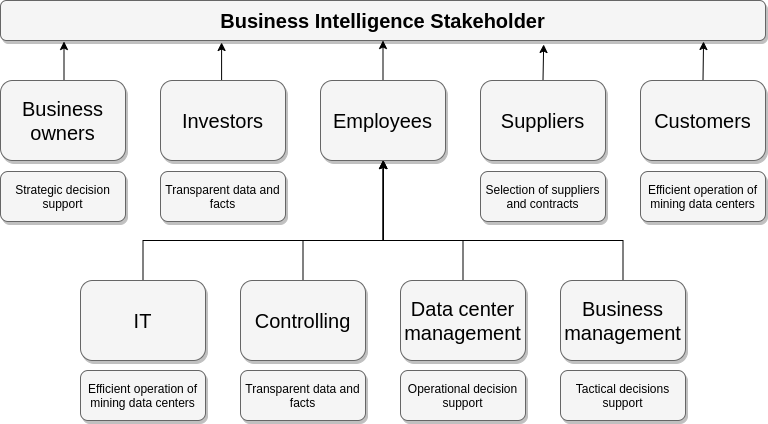
\includegraphics[width=0.8\textwidth]{internalstakeholder}
    \label{figure:internalstakeholder}
\end{figure}

Es existieren noch weitere Gruppen von Stakeholdern, die jedoch keinen Einfluss auf die \ac{BI} Auswertung haben.
Dazu zählen politische Gruppen, Regierungen und das Gemeinwesen.\footcite[Vgl.][Abb. 14.2]{simmers2004stakeholder}

\subsection{Planung des Business Intelligence Prozesses} \label{toc:planungdesbiprozesses}

Im folgenden Teil wird ein beispielhafter \ac{BI} Prozess in einem betrieblichen Umfeld geplant. Der Betrieb, für den dieser Prozess
geplant wird, ist die Genesis Group und ist bereits in Kapitel \ref{toc:motivation} beschrieben worden. Für die Planung werden
die Schlussfolgerungen aus Kapitel \ref{toc:ansatzmoeglichkeitenfuerbusinessintelligence} verwendet. Innerhalb der Genesis Group
wird für die IT Infrastruktur die Google Cloud verwendet, weshalb in den folgenden Kapiteln passende Beispielprodukte aus dieser Cloud
identifiziert werden.\footcite[Vgl.][]{googlecloud2021dw} Analog zu einem \ac{BI} Prozess ist die folgende Studie in die Schritte der Datenbeschaffung
(Kapitel \ref{toc:datenhaltung}), Datenanalyse (Kapitel \ref{toc:datenanalyse}) und Datenpräsentation (Kapitel \ref{toc:datenpraesentation})
unterteilt. Am Ende findet eine Bewertung der Studie statt, welche die Argumentation der Teilhypothesen aus Kapitel
\ref{toc:ansatzmoeglichkeitenfuerbusinessintelligence} mit prüft und gegebenenfalls ergänzt.

\subsubsection{Beschaffung der Daten} \label{toc:datenhaltung}

Als Datenquellen werden die in Kapitel \ref{toc:klassifizierungderdaten} aufgezeigten Schnittstellen und Systeme verwendet.
Wie aus Tabelle \ref{tbl:klassifizierunginternedaten} und \ref{tbl:klassifizierungexternedaten} hervorgeht, sind alle Datenquellen für die
Verwendung innerhalb eines \ac{BI} geeignet und können daher in dementsprechenden \ac{ETL} Pipelines verwendet werden.
Eine Möglichkeit \ac{ETL} Pipelines in der Cloud errichten zu können, ist die Verwendung des "`Cloud Data Fusion"'
Dienstes.\footcite[Vgl.][]{googlecloud2021dw} Dieser ist auf den Aufbau solcher Pipelines spezialisiert und bietet zudem Schnittstellen
zu einem Data Warehouse in der Cloud an. Das Data Warehouse an sich wird über den "`Big Query"' Dienst realisiert.\footcite[Vgl.][]{googlecloud2021dw}
Dieses Warehouse ist der zentrale Ort, an dem alle relevanten Daten für die Analysephase des \ac{BI} Prozesses gespeichert werden und
ist daher zusammen mit den \ac{ETL} Pipelines für den Aufbau von \ac{BI} nicht wegzudenken.\footcite[Vgl.][S. 105ff]{loshin2012business}
Das Data Warehouse wird über den "`Cloud Data Fusion"' Dienst befüllt. Nach diesem Schritt sind alle benötigten Daten intern
im eigenen Data Warehouse verfügbar. Deshalb ist anzunehmen,
dass die Erhebung und die Beschaffung von Daten unter Zuhilfenahme der Google Cloud möglich ist und die betriebliche
Umsetzung für diesen Schritt gegeben ist.

\subsubsection{Analyse der Daten} \label{toc:datenanalyse}

Für die Analyse der Daten, die nun in einem Data Warehouse vorliegen, werden die Analyseverfahren verwendet, die in
Kapitel \ref{toc:analyseverfahrenbi} beschrieben sind. In der Google Cloud liegen für die Realisierung dieser Verfahren
mehrere mögliche Produkte vor.\footcite[Vgl.][]{googlecloud2021dw} Dazu zählen das Produkt "`Looker"', das eine \ac{OLAP} Plattform für \ac{BI}
ist, der "`Dataflow"' Dienst, der Datensätze in Echtzeit sowie als Stapelverarbeitung analysiert und "`Dataproc"', welcher
unter anderem die Möglichkeit des Betriebes von Apache Spark bietet.\footcite[Vgl.][]{googlecloud2021dw} Alle diese Werkzeuge reichen aus, um die Analysephase
eines \ac{BI} Prozesses abbilden zu können. 

Das Resultat aus Kapitel \ref{toc:zusammenfassendebetrachtung} war, dass die Implementierung eines \ac{BI} Prozesses möglich ist, jedoch
Schwierigkeiten bei der Vorhersage des Bitcoin Tauschkurses vorliegen. Diese Problematik beschränkt sich nicht direkt auf Bitcoin
selbst, sondern ist für die Vorhersage jeglicher Börsenkurse der Fall. 
Eine Möglichkeit mit Vorhersagemodellen zu arbeiten, ist nicht die Vorhersage eines konkreten
Kurses, sondern die Bildung verschiedener Szenarien, die mögliche Reaktionen und Entscheidungen des Managements beinhalten.\footcite[Vgl.][]{appendix:mcpreis}
Eine passende Möglichkeit ist dabei die Anwendung stochastischer Modelle, insbesondere von Monte-Carlo-Simulationen.\footcite[Vgl.][S. 28]{cocco2016modeling}
Diese werden bereits für die Szenarienbildung in der Genesis Group verwendet. Die vorliegende Monte-Carlo-Simulation wurde
am 06.11.2020 angefertigt.\footcite[Vgl.][]{appendix:mcpreis} Bei dem Vergleich zu den realen Daten aus dieser Zeit ist bemerkbar, dass sich diese Form der Simulation
für Vorhersagenmodelle für die nahe Zukunft (< 1 Monat) eignet.\footcite[Vgl.][]{appendix:btcusd} Die weiteren Ereignisse waren maßgeblich durch Social Media
bestimmt und konnten daher nicht im Rahmen dieser Simulation abgebildet werden.
Diese Form der Simulation gibt die Möglichkeit,
beliebig viele mögliche Kursentwicklungen zu berechnen und statistisch
auszuwerten.\footcite[Vgl.][]{appendix:mcpreis}\footcite[Vgl.][]{appendix:mcszenarien} Dabei entstehen mehrere
Szenarien, die verschiedene Reaktionen des Managements implizieren. Die Ausgangswerte für eine solche Analyse
werden durch das Data Warehouse bereitgestellt. Die Ergebnisse
werden wiederum in das Data Warehouse eingetragen und sind somit auch für andere Analyseverfahren zugänglich. Wie allerdings bereits
in Kapitel \ref{toc:ansatzmoeglichkeitenfuerbusinessintelligence} festgestellt, haben beispielsweise Social Media Plattformen einen
großen Einfluss auf die Entwicklung des Bitcoin Kurses. Solche Entwicklungen können nicht direkt mit stochastischen Modellen dargestellt
werden. Hierbei ist wieder die Echtzeitverarbeitung der Daten wichtig, damit die bereits beschriebenen Stakeholder direkt reagieren können.
Zusätzlich zu der Entwicklung des Bitcoin Kurses ist es durch eine Monte-Carlo Simulation möglich, die Entwicklung der gesamten
Netzwerkhashrate des Bitcoin Netzwerks zu simulieren.\footcite[Vgl.][]{appendix:mchashrate}

Es ist feststellbar, dass durch den Wechsel von stengen Vorhersagemodellen auf eine gröbere Szenarienbildung
der vorhersagende Aspekt von \ac{BI} umgesetzt werden kann. Auch für die Teilhypothesen eins und drei ist prädiktive bzw.
präskriptive \ac{BI} möglich. Die betriebliche Umsetzbarkeit ist gegeben.

\subsubsection{Präsentation der Daten} \label{toc:datenpraesentation}

Dieser Teil beschäftigt sich mit dem Vorgang, wie nun das Wissen, das durch die passende Analyse der Daten generiert worden ist, den
relevanten Stakeholdern in der korrekten Art und Weise zugänglich gemacht wird und dadurch das Ziel der Entscheidungsunterstützung
erreicht wird. Dafür werden im Folgenden die Stakeholder aus Kapitel \ref{toc:stakeholderanalyse} betrachtet. Es existieren mehrere
Möglichkeiten, wie das Wissen diesen Personen und Gruppen zugänglich gemacht werden kann:\footcite[Vgl.][Kap. 19]{loshin2012business}
\begin{itemize}
    \item \textbf{Berichtswesen: }Dies ist die einfachste Form der Präsentation. Dabei werden
    statische Berichtsvorlagen konfiguriert, aus denen regelmäßig Berichte automatisiert erstellt werden und den Stakeholdern zur Verfügung
    gestellt werden.\footcite[Vgl.][S. 305]{loshin2012business} Beispiele für solche Berichte in dem Kontext dieser Arbeit sind Berichte über die Ausfallszeiten der Mining
    Hardware oder monatliche Zusammenfassungen der finanziellen Situation der Rechenzentren. Die Erstellung solcher Berichte kann in
    der Google Cloud über den "`Cloud Scheduler"' realisiert werden.\footcite[Vgl.][]{googlecloud2021scheduler} Den relevanten Stakeholdern können die Berichte dementsprechend
    aktiv (beispielsweise über E-Mail) oder passiv über Downloads zur Verfügung gestellt werden.
    \item \textbf{\ac{OLAP} und Ad-Hoc Suchen: }Bei dieser Form der Präsentation werden über ein \ac{OLAP} System eigene Suchanfragen erstellt
    und damit zugeschnittenes Wissen erzeugt.\footcite[Vgl.][S. 308f]{loshin2012business}
    Diese Suchanfragen können spontan (Ad-Hoc) über das \ac{OLAP} System erstellt werden
    und werden direkt dem Stakeholder zur Verfügung gestellt. Beispiele hierfür sind Anfragen, die den Neu- oder
    Ausbau von Mining Rechenzentren betreffen. Ein Beispiel für ein solches System ist der "`Looker"' Dienst der
    Google Cloud.\footcite[Vgl.][]{googlecloud2021dw}
    \item \textbf{Dashboards: }Eine weitere Methode, um das Wissen der Analyse Stakeholdern
    zur Verfügung zu stellen ist die Verwendung von Dashboards. Diese Dashboards
    können online aufgerufen werden und präsentieren Daten, die durch die unterliegende Software bezogen werden.\footcite[Vgl.][S. 314f]{loshin2012business} Gerade bei
    technischen \acp{KPI}, wie beispielsweise der Darstellung von Hashrates oder Stromverbrauch der Hardware, findet diese
    Form der Visualisierung Anwendung. Desweiteren sind die Stakeholder in der Lage, ihre eigenen Dashboards zu erstellen.\footcite[Vgl.][S. 314f]{loshin2012business}
    Eine gängige Anwendung zur Erstellung von Dashboards ist "`Grafana"'.\footnote{https://grafana.com}
    \item \textbf{Alarmierung: }Diese Methode sendet proaktiv Benachrichtigungen und Alarme an
    relevante Stakeholder.\footcite[Vgl.][S. 311f]{loshin2012business} Damit sind diese in der Lage, mit nur geringem Zeitversatz auf veränderte Umstände zu reagieren. Beispielsweise
    fällt der komplette Ausfall eines Rechenzentrums oder Abweichungen der Realität zu den Vorhersagemodellen unter die Fälle, in denen
    eine Alarmierung Sinn machen kann. Solche Alarme können dann über Mail oder Instant Messenger den betreffenden Stakeholdern zugestellt
    werden.\footcite[Vgl.][S. 311f]{loshin2012business} Ein Dienst, der die Erstellung solcher Alarme zulässt, ist der "`Pub/Sub"' Dienst.\footcite[Vgl.][]{googlecloud2021dw} Für das Senden von Alarmen
    können Überwachungssysteme, wie "`Prometheus"', zum Einsatz kommen.\footnote{https://prometheus.io}
\end{itemize}

Alle diese Formen der Präsentation sind ohne Weiteres innerbetrieblich durchführbar. Daher exisitieren für diesen Schritt keine innerbetrieblichen
Hindernisse für die Implementierung eines \ac{BI} Prozesses.

\subsection{Abschließende Bewertung} \label{toc:abschliessendebewertung}

In Kapitel \ref{toc:planungdesbiprozesses} wurde im Zuge einer kleinen Fallstudie besprochen, ob es möglich ist, einen \ac{BI} Prozess,
wie er in Kapitel \ref{toc:ansatzmoeglichkeitenfuerbusinessintelligence} aufgezeigt worden ist, innerbetrieblich realisieren zu können.
Um dies zu erreichen wurden die drei Hauptschritte eines \ac{BI} Prozesses, die Datenbeschaffung, -analyse und -präsentation, einzeln
besprochen und mögliche technische Lösungsansätze anhand des Beispiels der Google Cloud aufgezeigt.

Zusammenfassend kann festgestellt werden, dass keine Hindernisse vorliegen, die einer Einführung eines \ac{BI} Prozesses widersprechen.
Zusätzlich zur Argumenation aus Kapitel \ref{toc:ansatzmoeglichkeitenfuerbusinessintelligence} ist es möglich, dass der \ac{BI} Prozess
bis hin zum präskriptiven Paradigma durchführbar ist (Vgl. Tabelle \ref{tbl:hypothesenanalyse2}). Daher ist es ohne Einschränkung möglich, dass alle Teilhypothesen in einem
solchen Prozess abgebildet werden können. Dadurch ist im Rückschluss möglich zu sagen, dass die Haupthypothese dieser Arbeit bestätigt werden
kann. Mittels \ac{BI} ist es möglich, dass Kryptomining Rechenzentren finanziell optimiert werden können.

\begin{table}[H]
    \caption{Ergebnis der Durchführbarkeit eines Business Intelligence Prozesses}
    \label{tbl:hypothesenanalyse2}
    \begin{tabularx}{\textwidth}[ht]{X||c|c|c|c}
         & \ac{HT0.1} & \ac{HT0.2} & \ac{HT0.3} & \ac{HT0.4}  \\
        \hline\hline
        Deskriptive Analyse & \checkmark & \checkmark & \checkmark & \checkmark \\
        \hline
        Vorhersagende Analyse & \checkmark & \checkmark & \checkmark & \checkmark \\
        \hline
        Präskriptive Analyse & \checkmark & \checkmark & \checkmark & \checkmark \\
    \end{tabularx}
\end{table}

Ein exemplarischer \ac{BI} Prozess für das Beispiel der Genesis Group kann wie in Abbildung \ref{figure:internalbiprocess} abgebildet aussehen.

\begin{figure}[H]
    \caption{Konzeption eines BI Prozesses innerhalb der Genesis Group}
    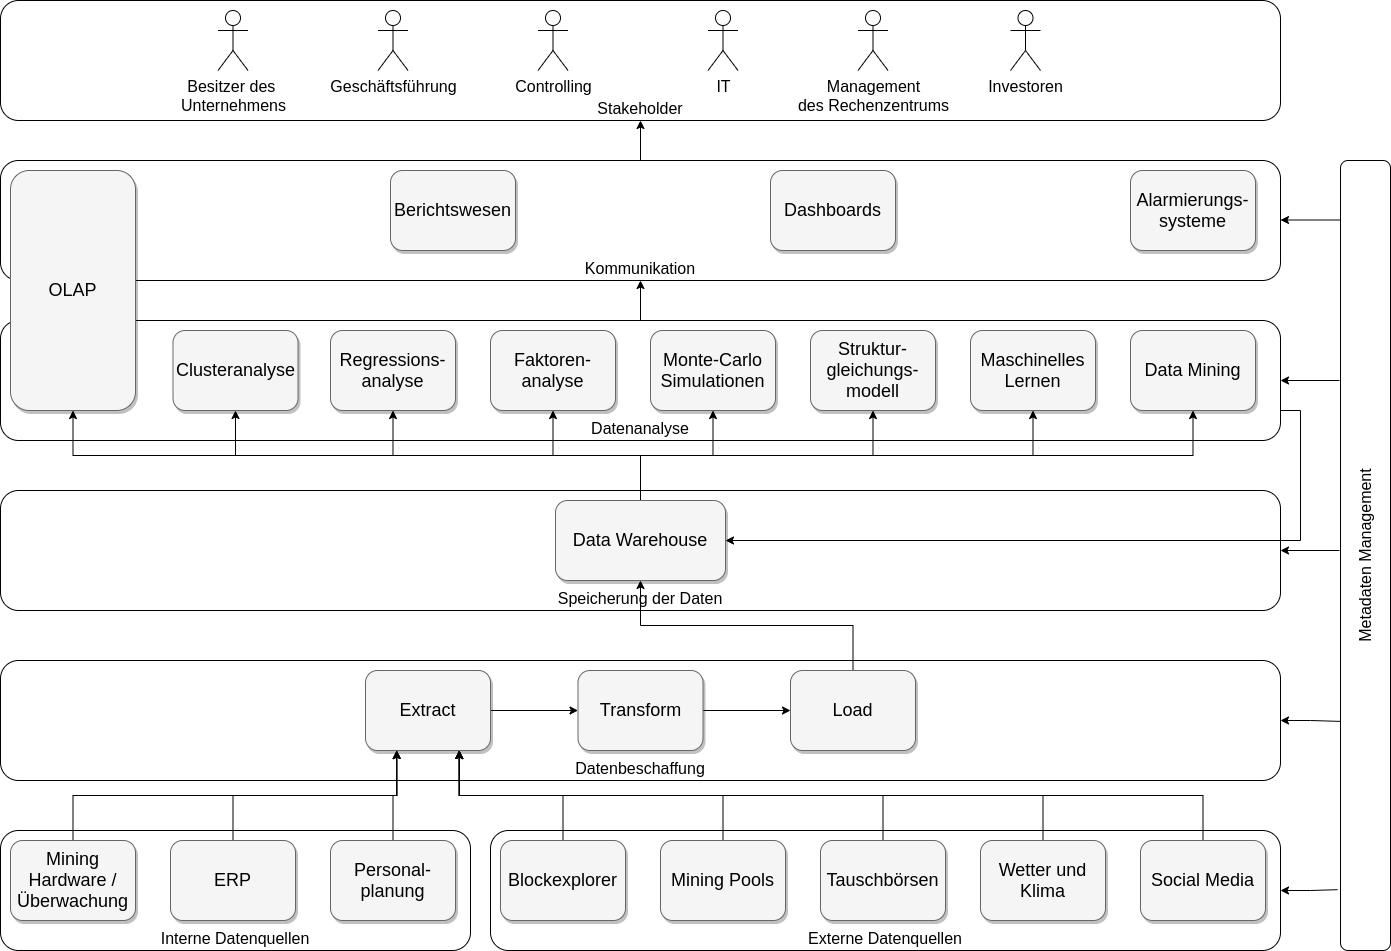
\includegraphics[width=\textwidth]{internalbiprocess}
    \label{figure:internalbiprocess}
\end{figure}

Diese Abbildung basiert prinzipiell auf dem Prozessaufbau, der in Kapitel \ref{toc:prozess} aufgezeigt ist, und teilt sich in die folgenden
Schritte auf:
\begin{itemize}
    \item \textbf{Datenquellen: }Als Datenquellen werden die Dienste, die in Kapitel \ref{toc:internedatenquellen} und \ref{toc:externedatenquellen}
    beschrieben werden, verwendet. Alle diese Quellen reichen zusammen aus, um genügend Daten bereitzustellen, damit die vier Teilhypothesen und
    dadurch die Haupthypothese bewiesen werden können.
    \item \textbf{Datenbeschaffung: }Bei der Beschaffung der Daten werden \ac{ETL} Pipelines eingesetzt, die die Daten an den Schnittstellen
    zu den Quellen abfragen, diese in das gewünschte Format transformieren und letztendlich in einem Data Warehouse ablegen. Wie
    in der Klassifizierung der Datenquellen aus Tabelle \ref{tbl:klassifizierunginternedaten} und \ref{tbl:klassifizierungexternedaten},
    sowie Kapitel \ref{toc:datenhaltung} ersichtlich ist, können die \ac{ETL} Pipelines ohne Hindernisse aufgebaut und realisiert werden.
    \item \textbf{Speicherung der Daten / Datenhaltung: }Im dritten Schritt werden die extrahierten und strukturierten Daten in ein Data Warehouse
    geladen. Dieses beinhaltet alle Daten, die weiterhin für den \ac{BI} Prozess wichtig sind, um Ergebnisse den Stakeholder präsentieren zu können.
    Dieser Teil ist, wie in Kapitel \ref{toc:datenhaltung} gezeigt, realisierbar.
    \item \textbf{Datenanalyse: }Die gespeicherten Daten werden folgend für die Analyse verwendet, um neues Wissen generieren zu können.
    Dabei gibt es eine Vielzahl verschiedener Ansätze für die Analyse von Daten, die vertieft in Kapitel \ref{toc:analyseverfahrenbi}
    besprochen worden sind. Diese werden verwendet, um das Optimierungspotential eines Kryptomining Rechenzentrums herauszufinden und
    mögliche Ansätze zur Umsetzung zu identifizieren. Alle diese Formen der Analyse können innerbetrieblich
    ohne Weiteres umgesetzt werden. Die genaue Ausgestaltung der Analysealgorithmen ist jedoch ein langwieriger und komplexer Prozess
    und wird nicht im Zuge dieser Arbeit besprochen, da in dieser Arbeit die grundsätzliche Möglichkeit der Implementierung besprochen wird.
    \item \textbf{Kommunikation / Präsentation: }Im letzten Schritt werden die Daten in einer Art und Weise präsentiert, 
    durch die die Stakeholder des \ac{BI} Prozesses Zugang zum Wissen erlangen und dieses weiterverwenden können.
    Relevante Formen der Präsentation sind in
    Kapitel \ref{toc:datenpraesentation} besprochen worden und reichen aus, damit die Stakeholder in optimaler Art und Weise durch den
    \ac{BI} Prozess unterstützt werden. Die Umsetzung dieser Ebene ist ohne Weiteres möglich.
\end{itemize}

Im folgenden Kapitel wird das Fazit aus diesem und dem letzten Kapitel einer kritischen Bewertung unterzogen, um
letztendlich die Antwort auf die Haupthypothese in den richtigen Kontext setzen zu können.
